\documentclass{article}
\title{CUDA Parallel Programming\\Homework 5}
\usepackage{graphicx}
\usepackage[UTF8]{ctex}
\usepackage{hyperref}
\usepackage{amsmath}
\CTEXoptions[today=old]
\author{40647007S 朱健愷}

\begin{document}
	\maketitle
	\section{Source codes}
	\subsection{File Layout}
	\begin{itemize}
		\item histogram\textunderscore1GPU/hist\textunderscore{1gpu}\textunderscore{gmem}.cu - Main code computed in CPU and GPU using global memory, it is used to calculate histogram of pseudo random number generated exponential distribution random number.
		\item histogram\textunderscore1GPU/hist\textunderscore{1gpu}\textunderscore{shmem}.cu - Main code computed in CPU and GPU using shared memory, it is used to calculate histogram of pseudo random number generated exponential distribution random number.
		\item Makefile - Script to auto generate executable from code.
		\item histogram\textunderscore1GPU/experiment.sh - Script to auto generate results of CPU, GPU using global memory, GPU using shared memory statistic result using different block size.
		\item histogram\textunderscore1GPU/result/block\textunderscore{CPU}/Output - Output CPU compute result of calculate histogram of pseudo random number generated exponential distribution random number.
		\item histogram\textunderscore1GPU/result/gm\textunderscore{block}\textunderscore*/Output\textunderscore* - Output GPU with global memory compute result of calculate histogram of pseudo random number generated exponential distribution random number, the suffix represented the block size.
		\item histogram\textunderscore1GPU/result/shm\textunderscore{block}\textunderscore*/Output\textunderscore* - Output GPU with shared memory compute result of calculate histogram of pseudo random number generated exponential distribution random number, the suffix represented the block size.
		\item notebook/*.png - Plots concluding output result
	\end{itemize}
	
	
	\subsection{Usage}
	Make code in both histogram\textunderscore{1GPU}/ directory
	Run the experiment.sh script in histogram\textunderscore{1GPU}/ directory 
	
	\begin{verbatim}
	cd histogram_NGPU
	make
	sh experiment.sh
	\end{verbatim}
	
	And it will produce generating exponential distribution random number statistical result using different block size.

	\section{Result}
	\subsection{Experiment environment}
	I ran my code on workstation provided in course, below is the Setup of workstation
	\begin{itemize}
		\item Operating system: Linux version 4.19.172 (root@twcp1)\\(gcc version 6.3.0 20170516 (Debian 6.3.0-18+deb9u1))
		\item CPU: Intel(R) Core(TM) i7-4790 CPU @ 3.60GHz
		\item GPU: Nvidia GTX 1060 6GB
		\item Memory: 32GB 
	\end{itemize}
	\subsection{Performance}
	Below two figures showed GPU using global memory case and GPU using shared memory case generating random sample in exponential distribution fixing grid size and change block size.
	\begin{figure}[hb!]
		\centering
		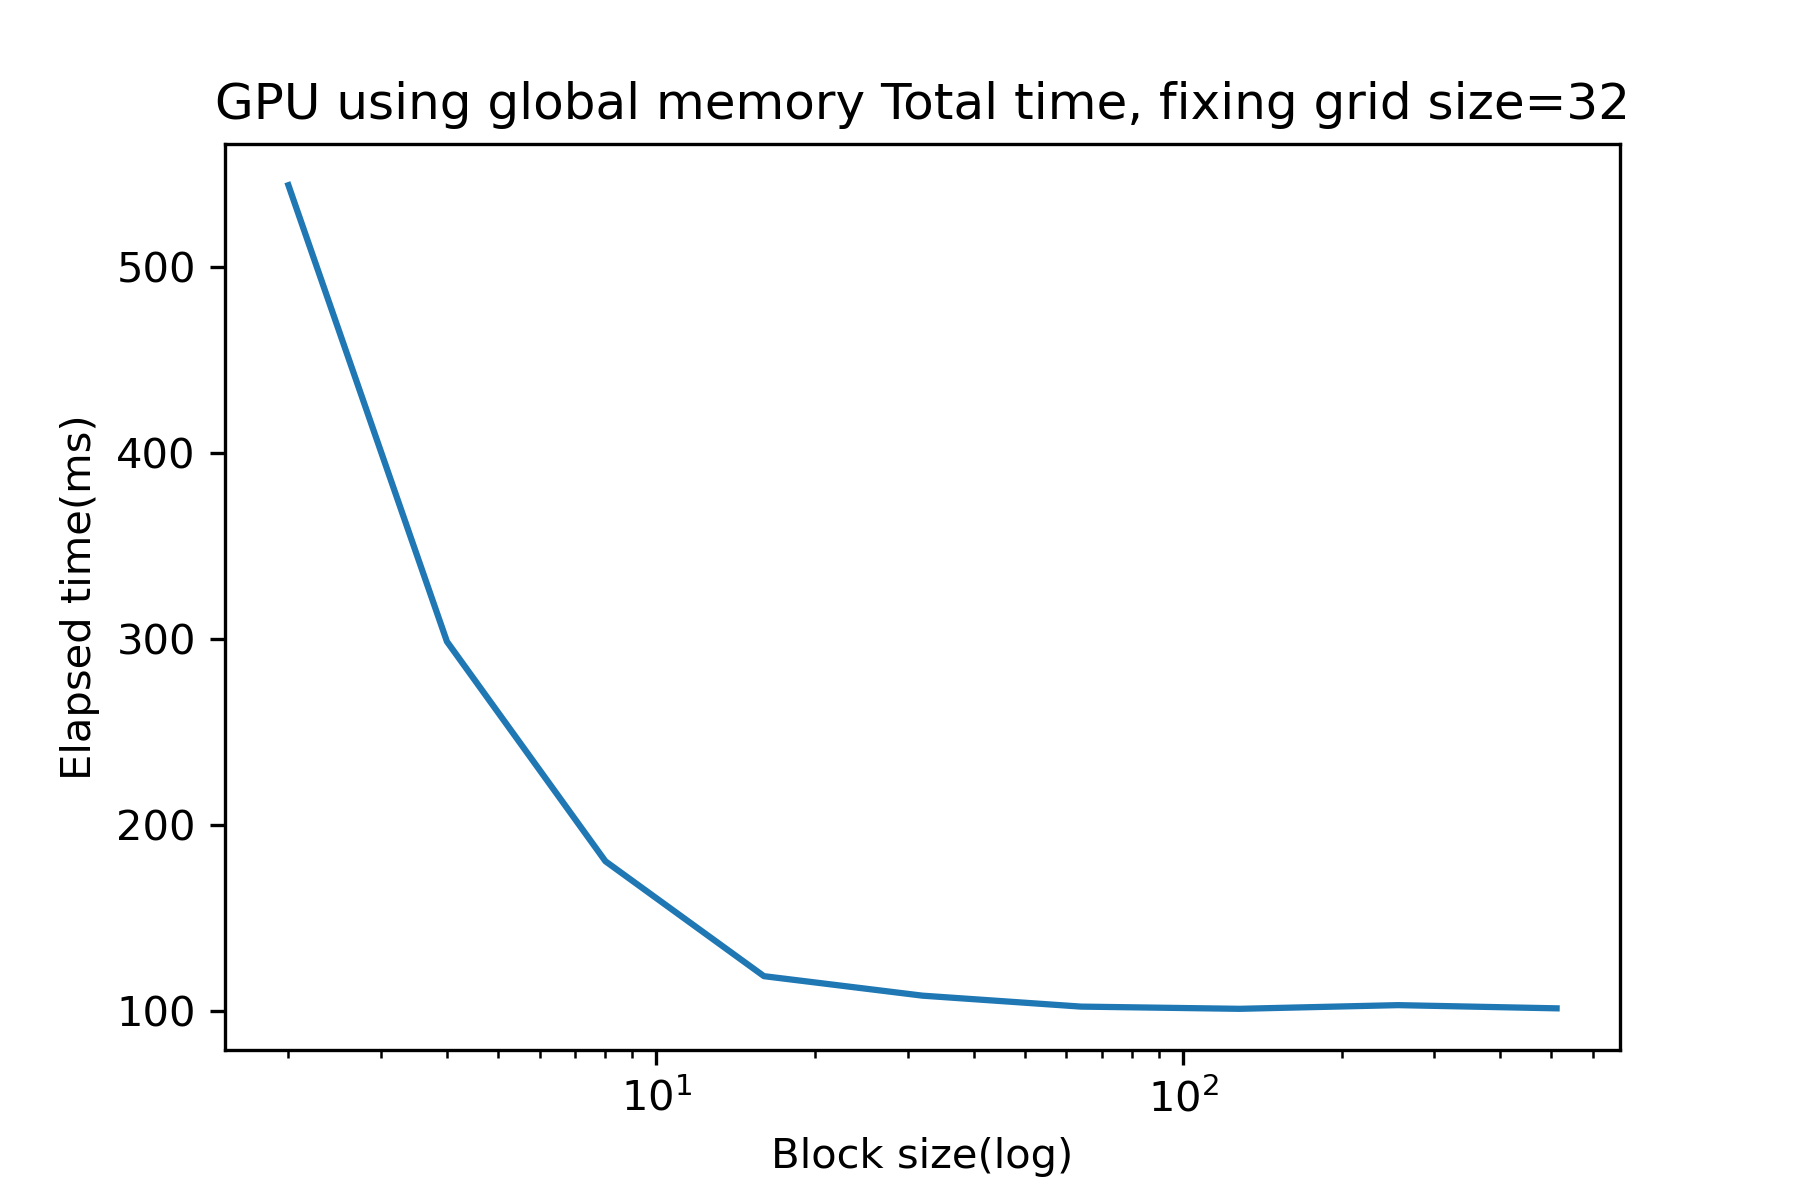
\includegraphics[width=\linewidth]{notebook/gpu_gmem_total_time_fix_grid}
	\end{figure}
	\begin{figure}
		\centering
		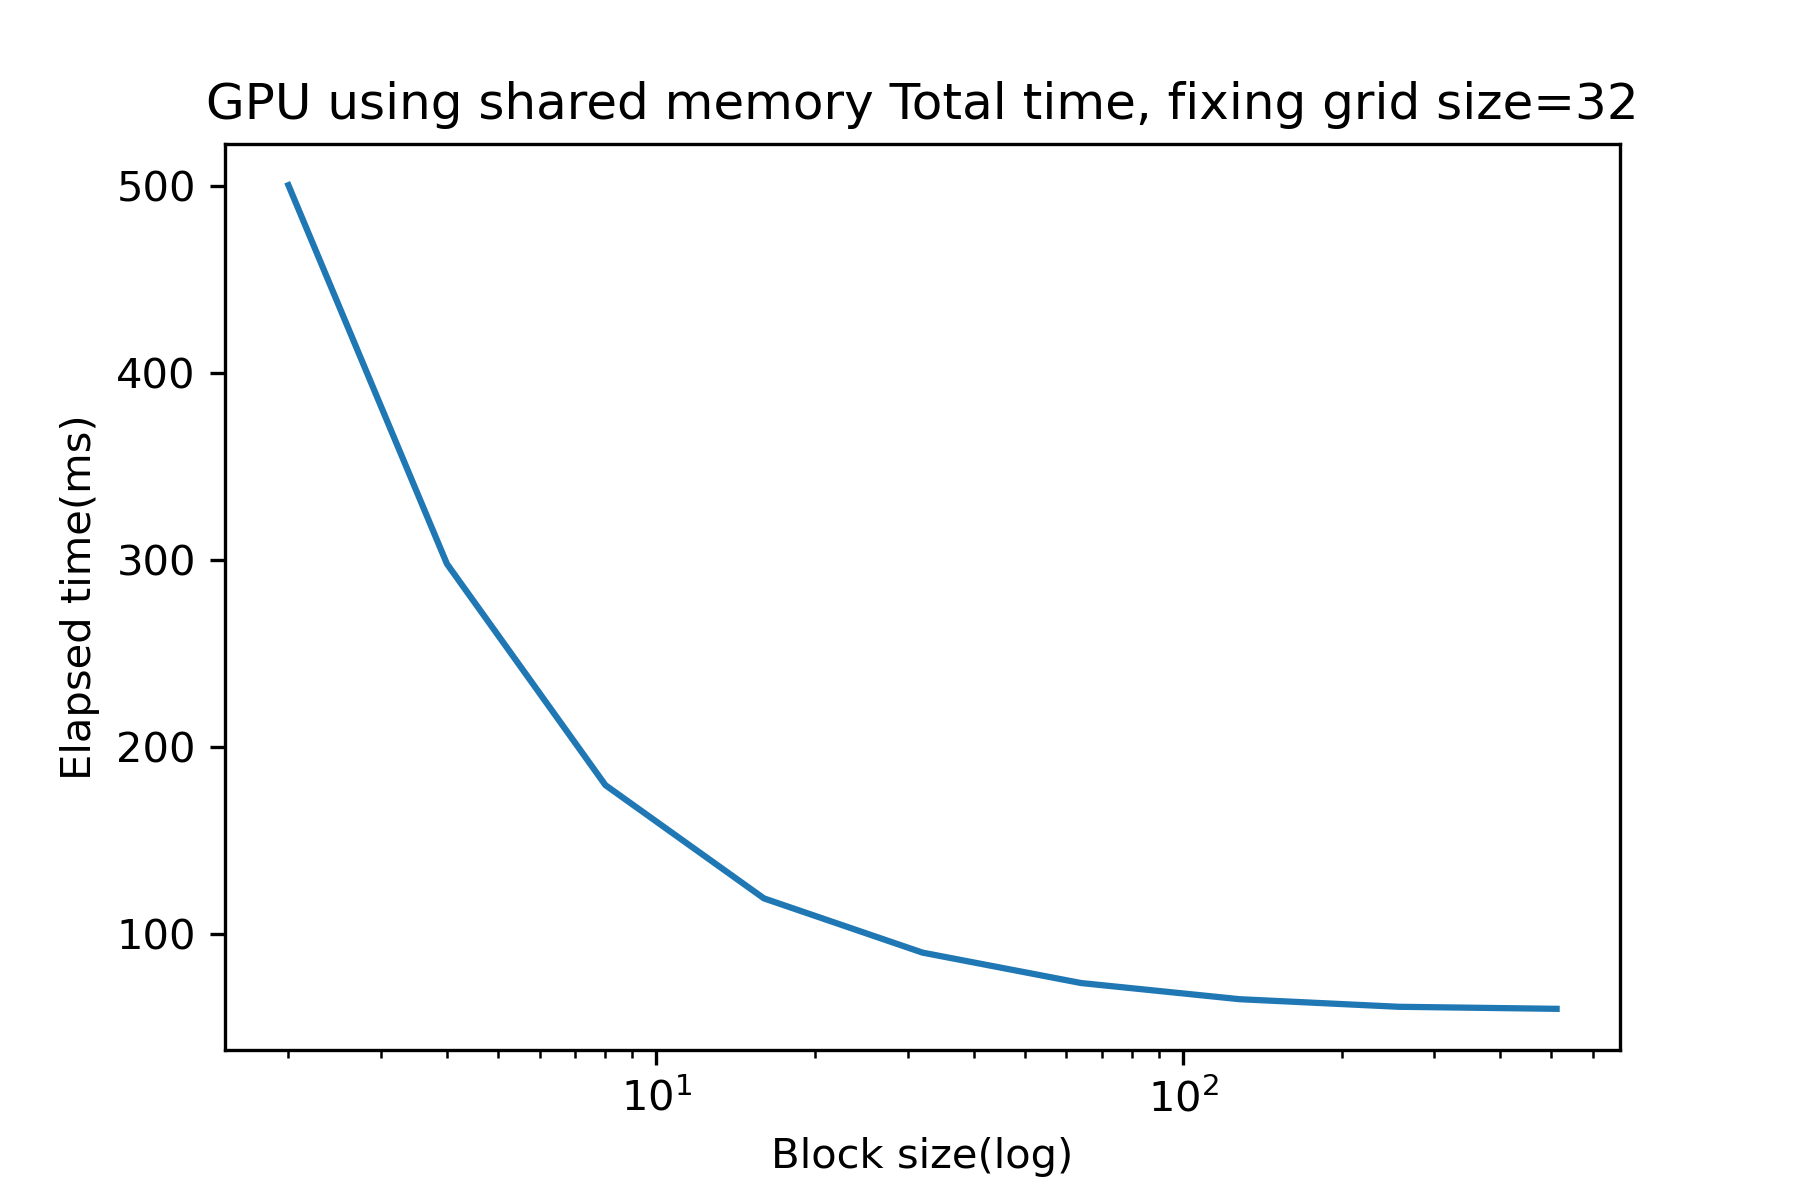
\includegraphics[width=\linewidth]{notebook/gpu_shmem_total_time_fix_grid}
	\end{figure}
	\newpage
	The CPU total time of generating random sample in exponential distribution is 156.274750 (ms).
	
	And below one figure showed the comparison between the generated random sample in exponential distribution and real exponential distribution.
	\begin{figure}[hb!]
		\centering
		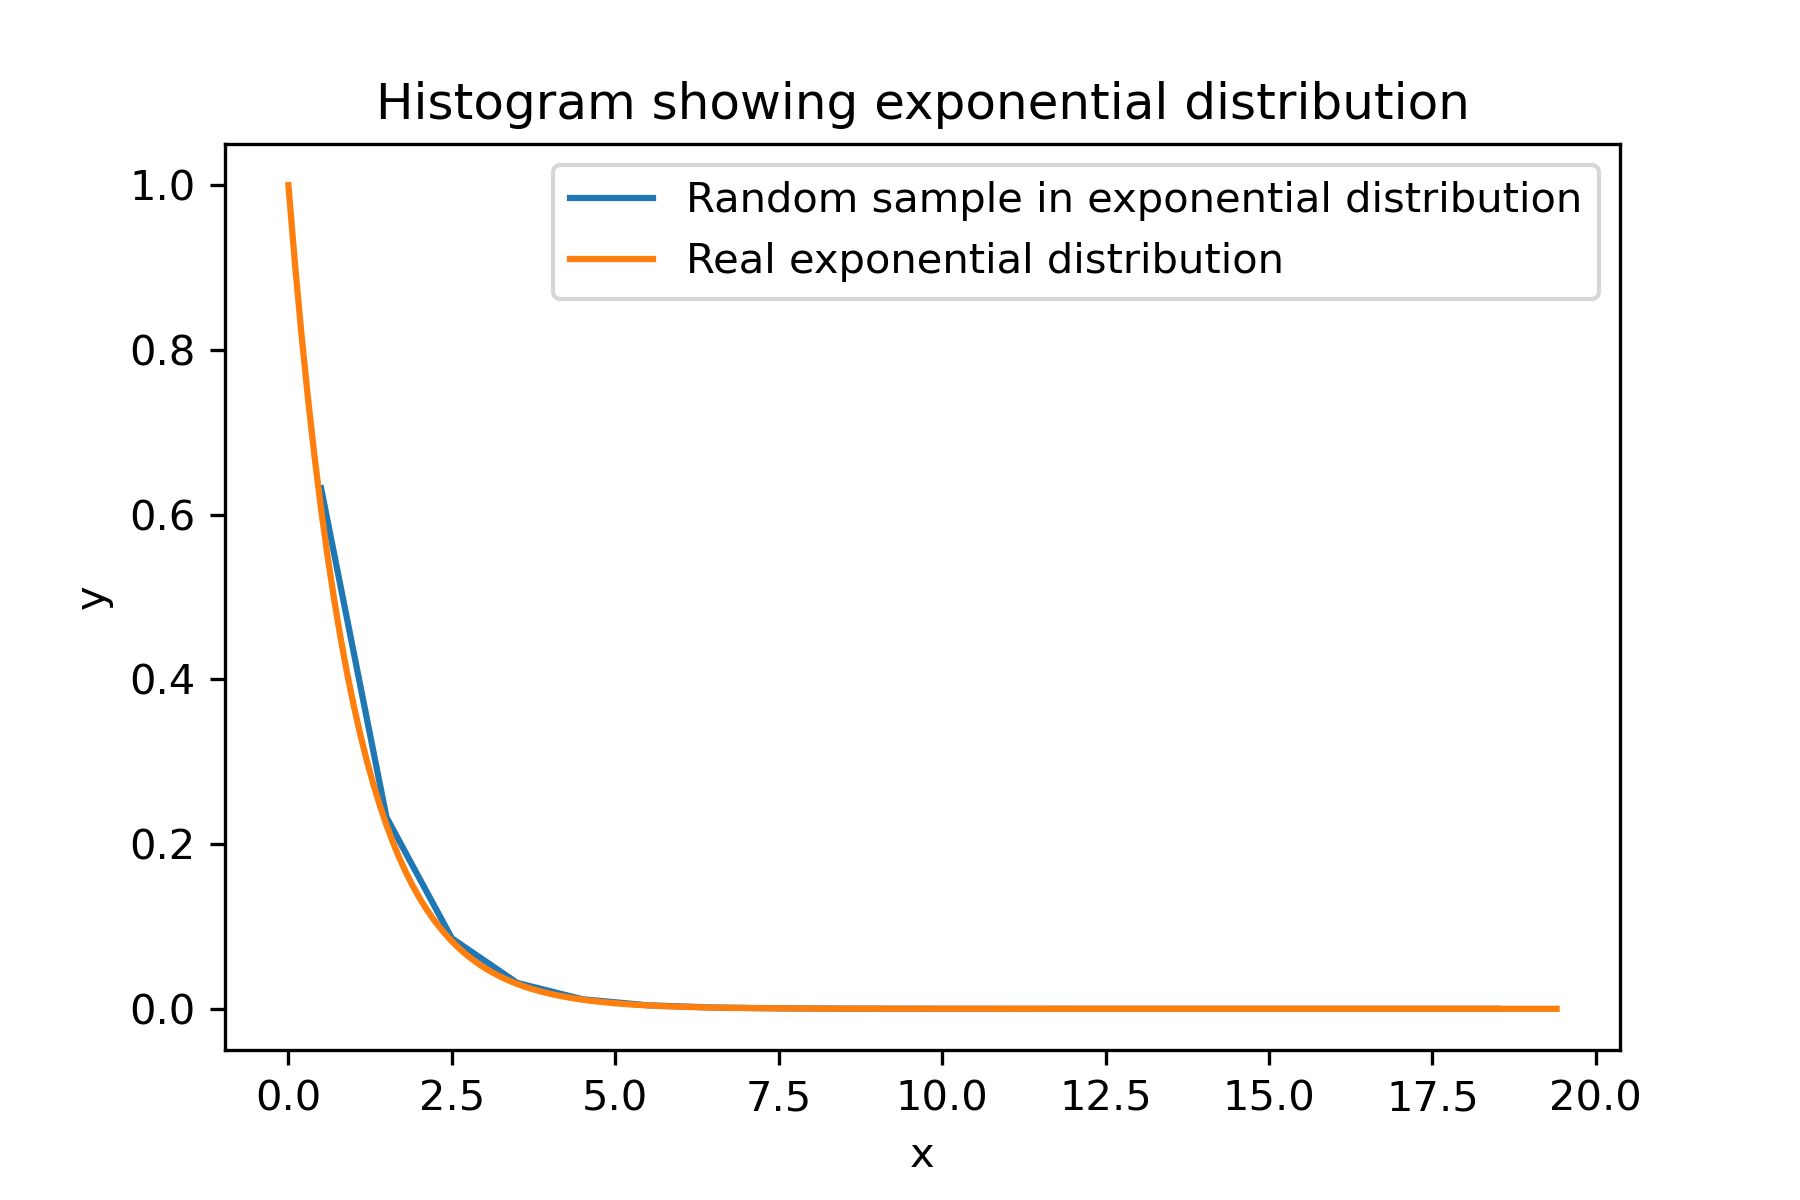
\includegraphics[width=\linewidth]{notebook/histogram}
	\end{figure}

	\subsubsection{Observation}
	We can observe that the performance of small block size setup in both GPU using global memory case and GPU using shared memory case yield the worse performance in my experiment. This may because of we don't have enough threads in grid to collect histogram datas which range are out of basic per threads in grid(namely, more loop is needed in while loop in device code). So the block size do affect the performance a lot.
	
	The result of utilizing shared memory helps improve the performance in nearly every block size setup. 
	
	The optimal block size setup of generating random sample in exponential distribution in my experiment is 128 block size for GPU using global memory case, 512 block size for GPU using shared memory case.
	
	\section{Discussion}
	The speed up of GPU using shared memory version compared to GPU using global memory version may due to the shared memory version first collect histogram data in shared memory, and then collect them to global memory, which largely decrease the time to wait the other threads to perform the atomic operations (namely write to same histogram bins).
\end{document}